\documentclass[11pt,a4paper]{article}
\usepackage[margin=2cm]{geometry}
\usepackage{graphicx,xcolor,enumitem,booktabs}
\usepackage[hidelinks]{hyperref}
\usepackage{parskip}
\graphicspath{{img/}}
\definecolor{ink2}{HTML}{52514E}
\renewcommand{\familydefault}{\sfdefault}
\setlist{nosep,leftmargin=1.4em}

\begin{document}
{\LARGE\bfseries FabricInspect-IoT -- Quick Guide}\\[2pt]
{\color{ink2} Fabric defect inspection that learns a new fabric from a few seconds of good material.
\url{https://github.com/nasin0764-bit/FabricInspect-IoT}}

\section*{What it does}
A camera looks at the fabric just before it reaches the seaming machine. The app learns what the
\emph{good} fabric looks like from about 10 frames and then flags every frame that looks different:
holes, cuts, threads, stains, contamination. It needs \textbf{no defect examples, no labelling, no GPU},
and it sets its own alarm threshold.

\begin{center}
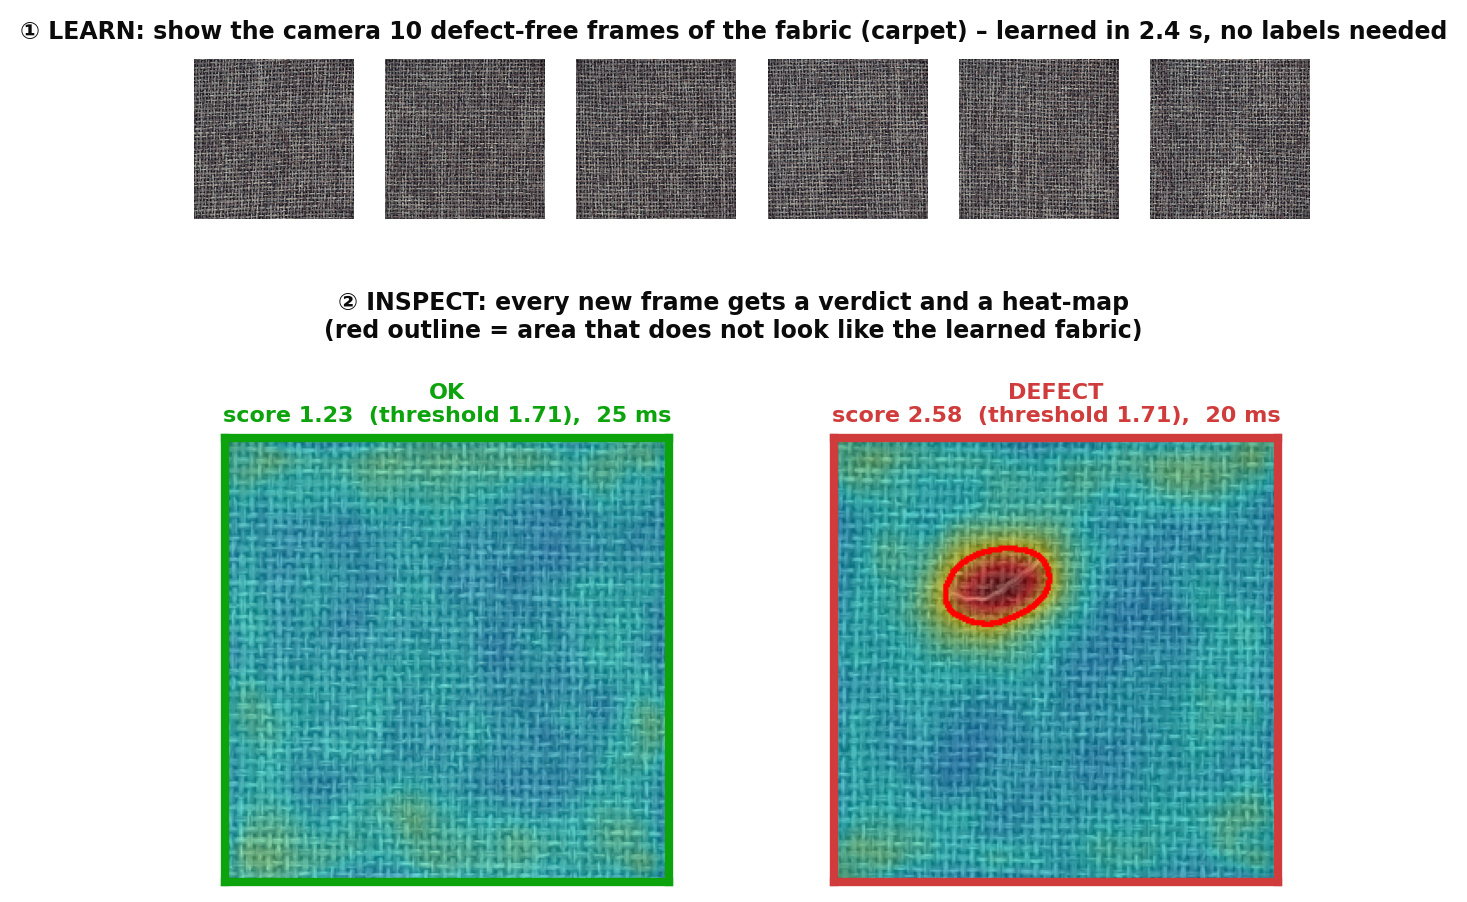
\includegraphics[width=0.9\textwidth]{guide_learn_inspect.png}
\end{center}

\section*{How to use it (single machine)}
\begin{enumerate}
\item Install once: \texttt{pip install -r requirements.txt}
\item Start the app: \texttt{python -m fabricinspect gui}
\item Click \textbf{Open camera} (or \textbf{Image folder\ldots}).
\item Type the fabric name, keep \emph{Good shots = 10}, click \textbf{Learn fabric}, and slowly move
      defect-free fabric under the camera. The model and its threshold are saved as a profile.
\item Click \textbf{Start inspection}. Each frame shows \textcolor[HTML]{0CA30C}{\textbf{OK}} or
      \textcolor[HTML]{D03B3B}{\textbf{DEFECT}} with a heat-map. Defect frames are saved and every
      decision is written to a CSV log in \texttt{\textasciitilde/FabricInspect/logs}.
\item Next time the same fabric comes back, choose it under \textbf{Profile} and click \textbf{Load}.
\end{enumerate}
Two detectors are available: \emph{Deep (PatchCore-lite)}, more accurate, and \emph{Light (Gabor-Gaussian)},
a 6\,kB model that runs on any small computer.

\section*{What the results look like}
Real outputs of the app on public test images (10 good frames learned per material). Five of these six
defects are found; the faint wood scratch is missed. The app is not perfect, and the threshold can be
made stricter or looser (\emph{margin} setting).
\begin{center}
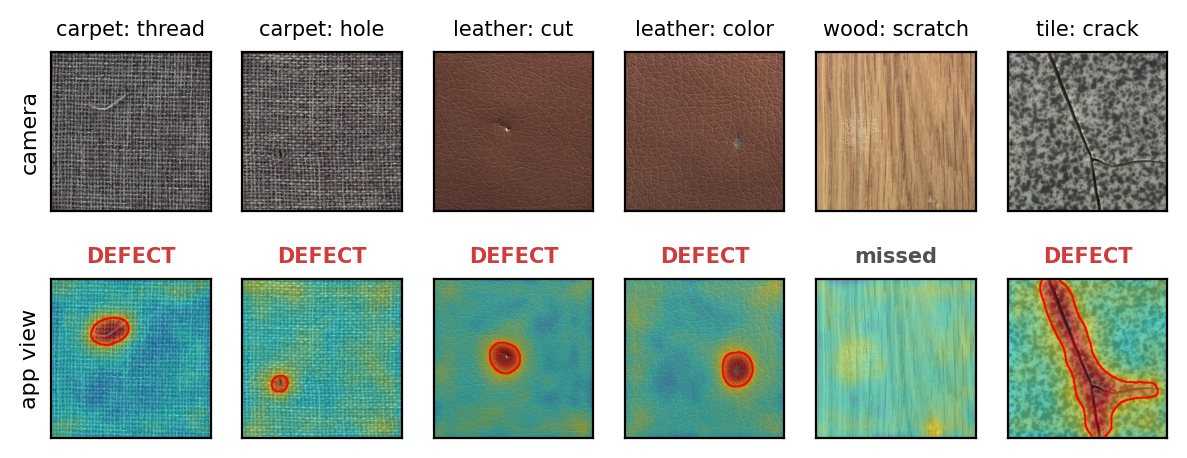
\includegraphics[width=\textwidth]{guide_gallery.png}
\end{center}

\section*{Many machines: the IoT mode}
\begin{minipage}[t]{0.47\textwidth}\vspace{0pt}
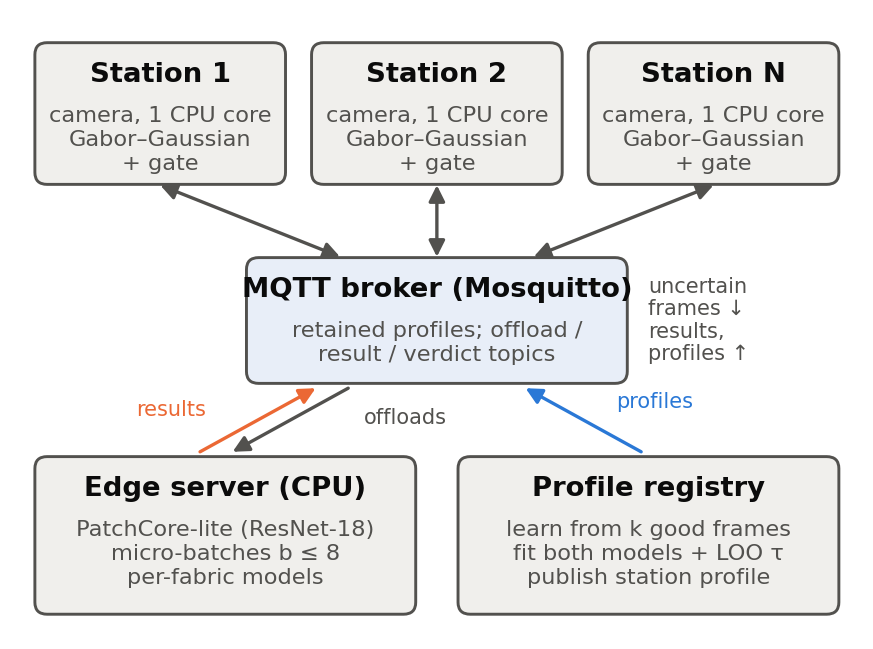
\includegraphics[width=\textwidth]{fig_architecture.png}
\end{minipage}\hfill
\begin{minipage}[t]{0.5\textwidth}\vspace{0pt}
\begin{itemize}
\item \textbf{Stations} (one per machine) run the light model and decide clear cases themselves in about 40\,ms.
\item Only \textbf{uncertain} frames are sent over MQTT to one \textbf{edge server}, which checks them with the deep model.
\item A fabric learned once is pushed by the \textbf{profile registry} to all machines within about 15\,ms.
\end{itemize}
\end{minipage}

\vspace{4pt}
\begin{verbatim}
mosquitto -p 1883                                          # message broker
python -m fabricinspect edge    --host <broker>            # edge server
python -m fabricinspect publish --host <broker> --name denim --images good_frames/
python -m fabricinspect station --host <broker> --name st01 --fabric denim --camera 0
\end{verbatim}

\section*{Why the gate matters}
\begin{minipage}[t]{0.45\textwidth}\vspace{0pt}
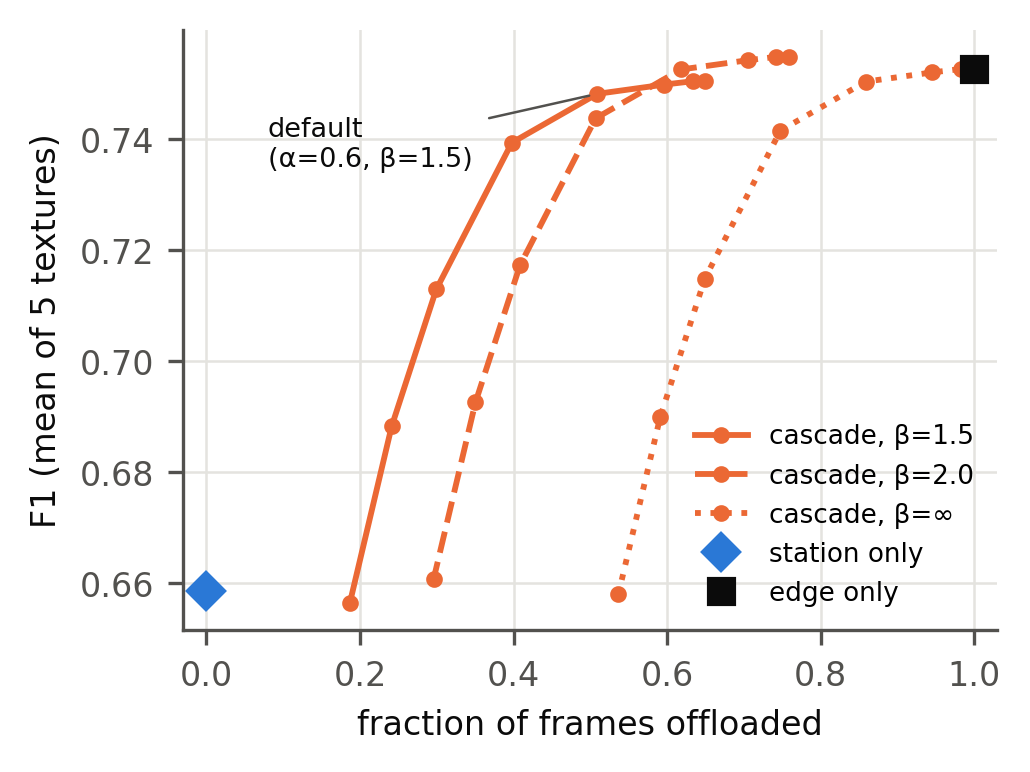
\includegraphics[width=\textwidth]{fig_gate.png}
\end{minipage}\hfill
\begin{minipage}[t]{0.52\textwidth}\vspace{0pt}
Sending every frame to the edge gives the best accuracy but loads the network and the server.
The \emph{confidence gate} keeps \textbf{99\,\% of that accuracy while sending only half the frames},
and sends more frames for hard fabrics (carpet: 81\,\%) and fewer for easy ones (leather: 23\,\%),
automatically.
\end{minipage}

\begin{center}
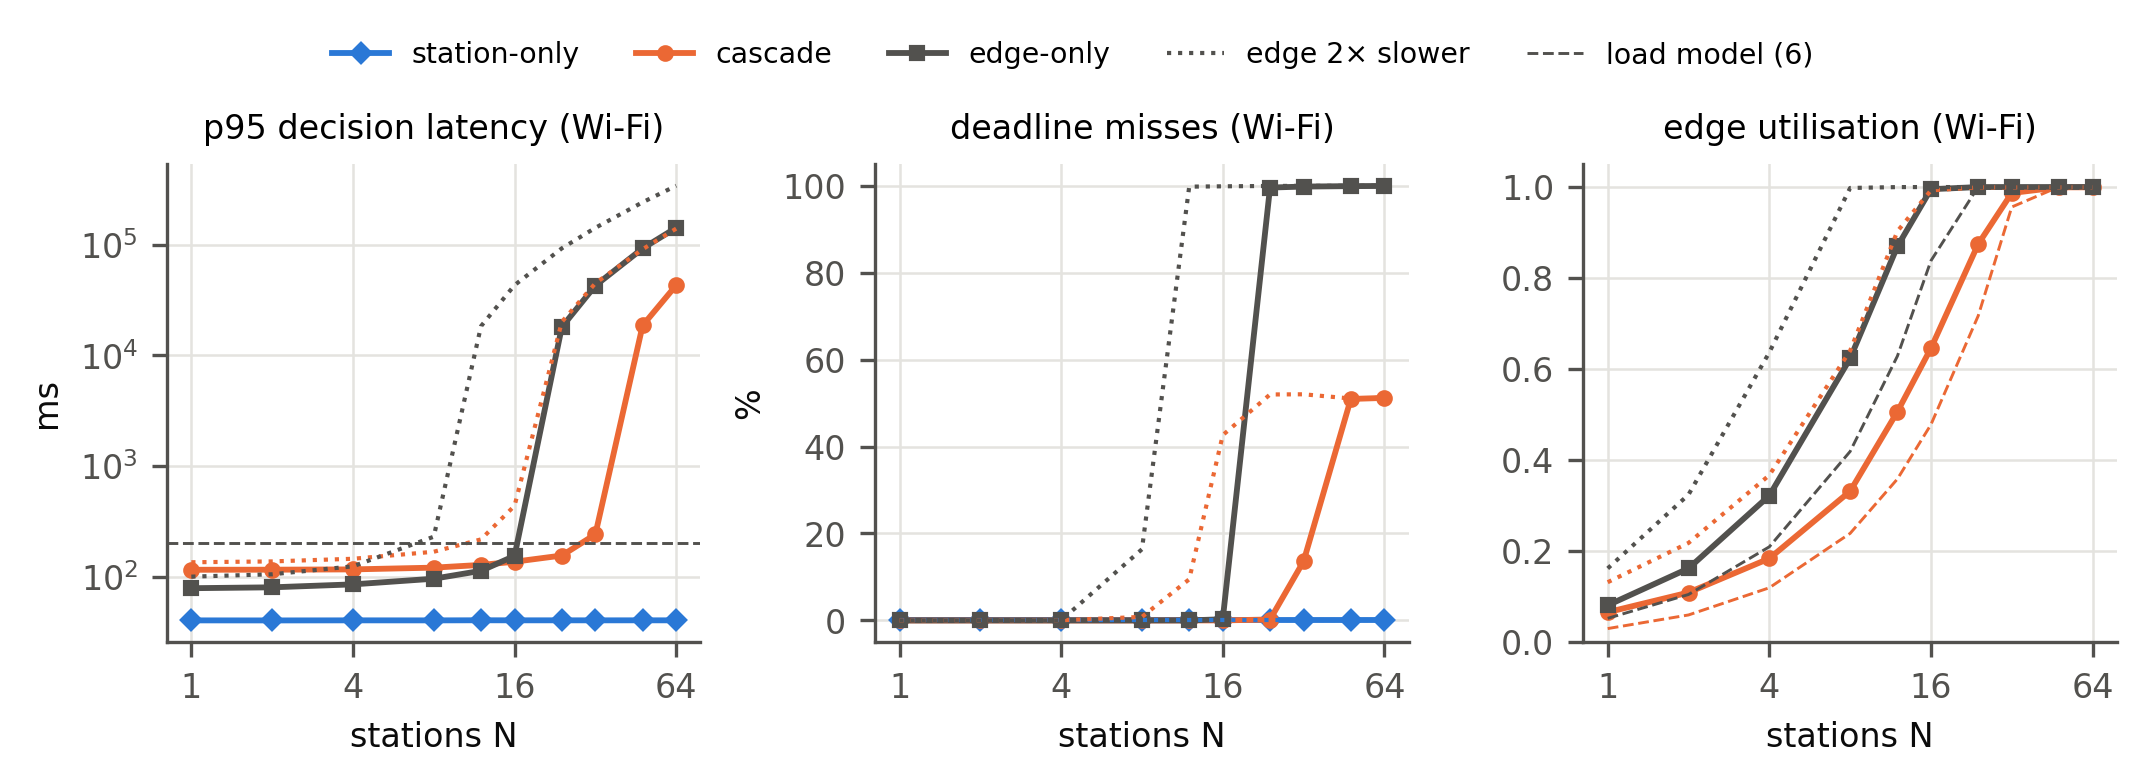
\includegraphics[width=\textwidth]{fig_sim.png}
\end{center}
With the gate, one ordinary PC as edge server answers within the 200-ms frame time for
\textbf{24 machines instead of 16}, and each machine sends 39\,\% less data.
(Simulation built from measured timings and checked against a live test bed; see the paper.)

\section*{Good to know}
\begin{itemize}
\item Re-learn the fabric after changing light, focus or camera; it takes seconds.
\item On a slow network (about 1\,Mbit/s) only the stations' own decisions arrive in time; offloaded
      frames are still checked, but later.
\item Very fine regular meshes (like the \emph{grid} test material) need more than 10 good frames.
\end{itemize}
\end{document}
